%% content.tex
%%

%% ==============
\chapter{Grundlagen}
\label{ch:Grundlagen}
%% ==============
\section{Rasterelektronenmikroskop}
\label{ch:Grundlagen:sec:REM}
In Abbildung \ref{fig:aufbau_rem} ist schematisch der Aufbau eines Rasterelektronenmikroskops~(REM) dargestellt. Aus in einer Elektronenquelle werden durch eine Spannung $U_{B}$ von einigen kV Elektronen (Prim"ar Elektronen - PE) aus einer Kathode gel"ost und beschleunigt. Durch ein System aus Magnetlinsen, Ablenkspulen und Blenden wird ein Elektronenstrahl geformt, mit dem die eine Probe abgetastet werden kann.

Treffen PE auf die Probe werden diese durch elastische oder inelastische Streuung abgebremst. Hierdurch werden von der Oberfl"ache durch verschiedene Prozesse Teilchen emittiert, die sich in ihrer Energie unterscheiden.

Bei Elektronen mit einer Energie von weniger als 50~eV spricht man von Sekund"arelektronen~(SE). Diese werden durch inelastische St"o"se der PE mit schwach gebunden Elektronen im Material erzeugt. Seitlich der Probe ist ein Everhart-Thornley-Detektor angebracht. Dieser beschleunigt durch eine Spannung die SE auf einen Szintilationskristall. Trifft ein Elektron auf diesen Kristall sendet er einen Lichtpuls aus, der anschlie"send durch einen Photomultiplier verst"arkt wird und in einen Spannungsimpuls umgewandelt werden. Es k"onnen nur SE detektiert werden, die im oberfl"achennahen Bereich des Materials erzeugt wurden (Vgl. Abb. \ref{fig:ionisationsbirne}), da die Energie der Elektronen nicht ausreicht, um das Material zu durchdringen \todo{hmm, bl"od}. Mit SE kann daher die Topografie des Materials mit hoher Aufl"osung vermessen werden.


Elektronen die Tiefer in das Material eindringen und stark vom Material gestreut werden, werden als R"uckstreuelektronen (engl. \textit{Backscattered Electrons} - BSE) bezeichnet. BSE besitzen eine Energie zwischen 50~eV und $ e \cdot U_B$. Sie werden durch einen Detektor, der "uber der Probe um die Apperturblende angebracht ist, detektiert (Vgl. Abb. \ref{fig:aufbau_rem}). Da die Streuung der Elektronen und damit die Energieverteilung der BSE von der Dichte des Untersuchten Materials abh"angt, lassen sich "uber BSE gut Materialkontraste darstellen. Allerdings ist die Aufl"osung geringer als bei SE.

Durch die



\begin{figure}
\centering
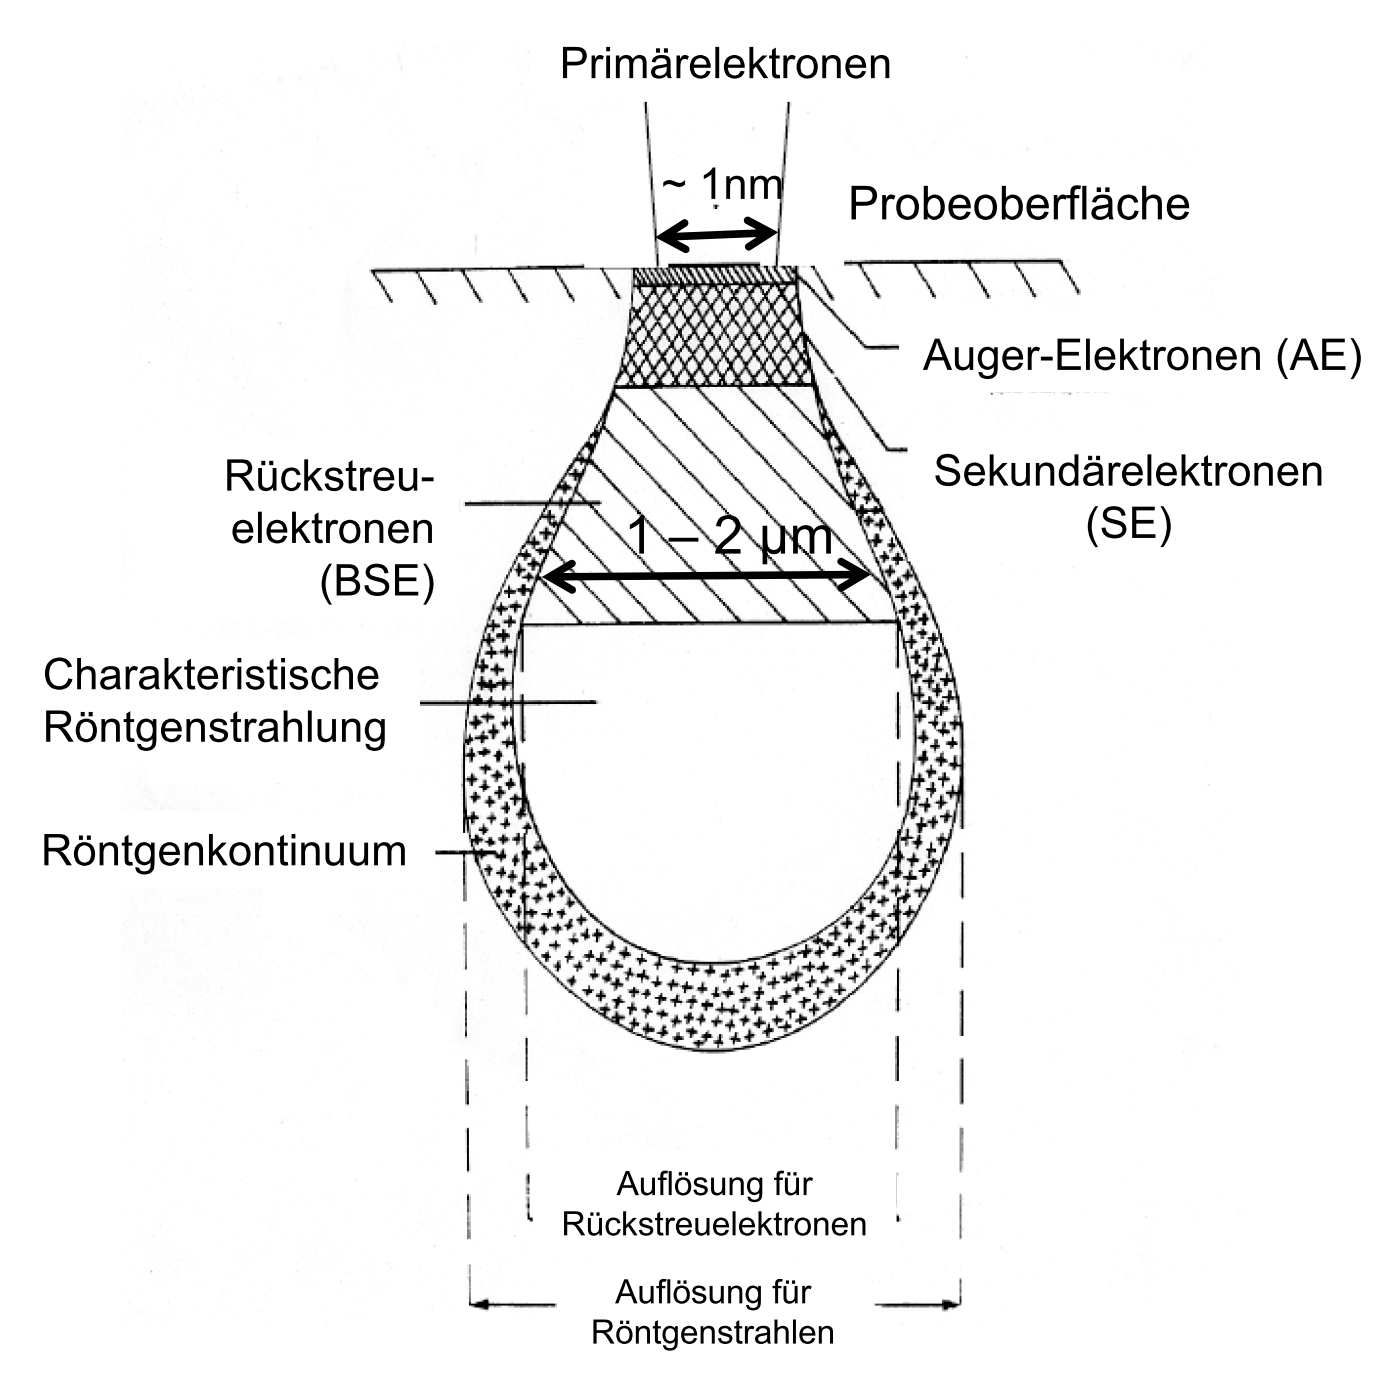
\includegraphics[width=.5\columnwidth]{Grafiken/ionisationsbirne.jpg}%
\caption{Ionisationsbirne \cite{Reimer}.}
\label{fig:ionisationsbirne}
\end{figure} 

\begin{figure}
\centering
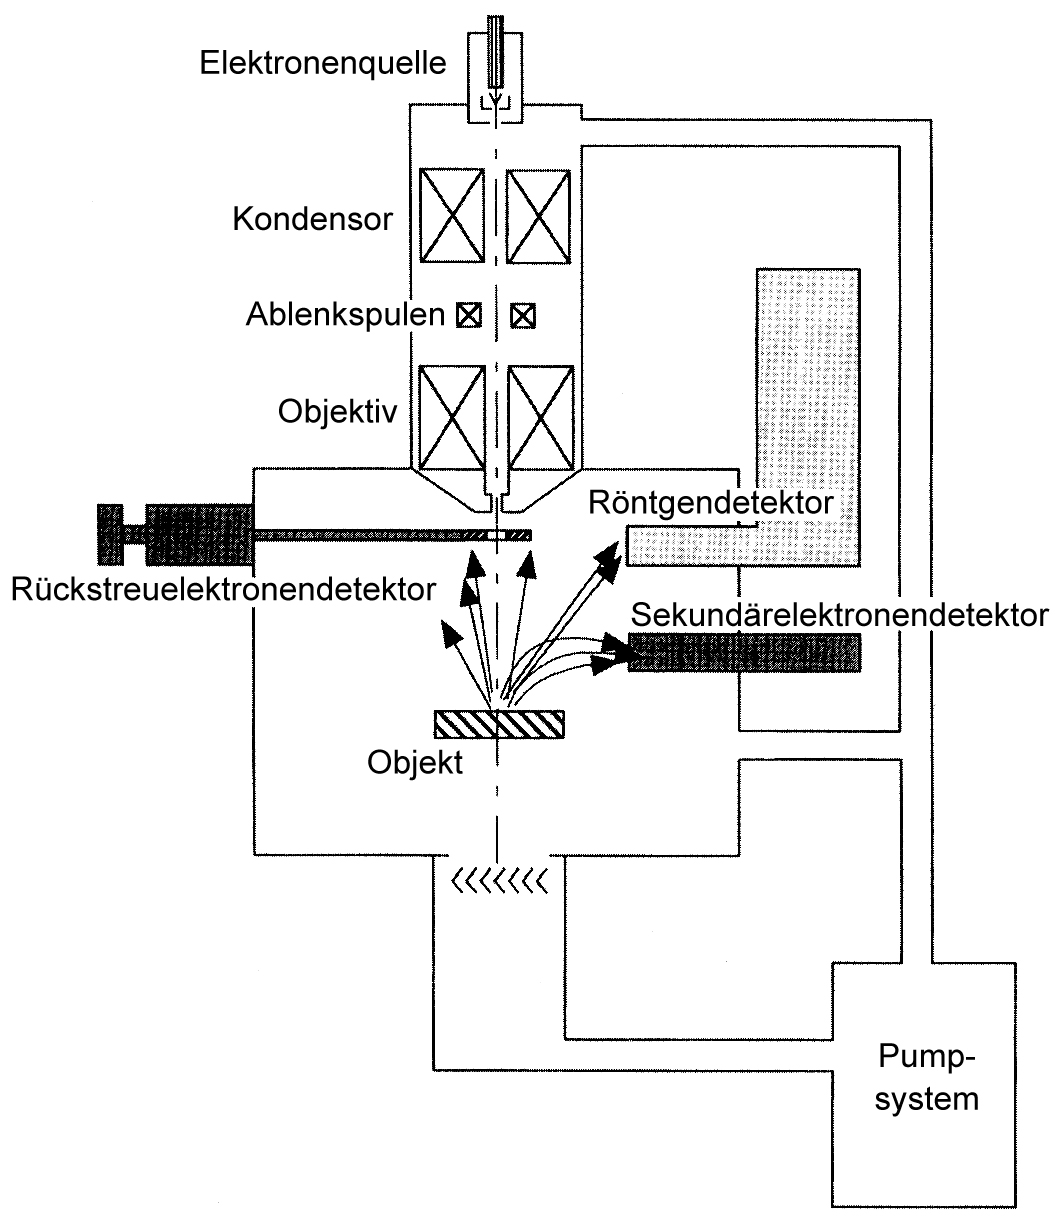
\includegraphics[width=.5\columnwidth]{Grafiken/rem-schema-1.jpg}%
 
\caption{Schematischer Aufbau eines REMs \cite{Colliex}.}
\label{fig:aufbau_rem}
\end{figure} 

\subsection{Aufbau}
\label{ch:Grundlagen:sec:REM:sub:Aufbau}

\subsection{Aufl�sungsverm�gen}
\label{ch:Grundlagen:sec:REM:sub:Aufl�sung}

\subsection{Tiefensch�rfe}
\label{ch:Grundlagen:sec:REM:sub:Tiefenschaerfe}

\section{Direct Laser Writing}
\label{ch:DLW}

\section{Aufbau und Funktionsweise}
\label{ch:DLW:sec:Aufbau}

\section{Noch eine}
\label{ch:DLW:sec:bla}

%% ===========================
\chapter{Versuchsdurchf�hrung}
\label{ch:Durchfuerhung}

\section{Probenherstellung}
\label{ch:Durchfuerhung:sec:Herstellung}

Zur Herstellung der Proben wurde auf ein gereinigtes Glassubstrat mit einem \textit{Spin Coater} ein Fotolackfilm (SU-8) aufebracht. Um das L�sungsmittel aus dem Lack zu treiben, wurde die Probe bei 95~�C auf einer \textit{Hot Plate} gebacken (\textit{Soft Bake}) \cite{Versuchsanleitung}. Diese Probenvorbereitung erfolgte durch den Versuchsbetreuer.

\todo{Schreiben der Probe im DLW}

Nach der Belichtun des Fotolacks erfolgte ein $Post~Exposure~Bake$ (PEB) f�r 7 Minuten bei 95~�C auf einer $Hot~Plate$. Bei diesem Backvorgang werden zuvor belichtete Bereiche des Lacks quervernetzt und damit unempfindlich gegen�ber dem Entwickler. Anschlie�end erfolgte die Entwicklung mit dem Entwickler \mbox{mr-Dev 600}. 
Die Probe wurde f�r 7 Minuten im Entwickler geschwenkt, zum stoppen der Entwicklung mit Isopropanol abgesp�hlt und mit Stickstoff getrocknet. Nach einer optischen Kontrolle der Probe wurde die Probe f�r eine weitere Minute in \mbox{mr-Dev 600} nachentwickelt. Bei der Entwicklung werden die zuvor nicht belichteten Lackbereiche entfernt.

Um die Lackstrukturen weiter zu festigen wurde die Probe f�r 10 Minuten bei 150~�C auf einer $Hot~Plate$ gebacken ($Hard Bake$). Bei diesem $Hard~Bake$ werden au�erdem Isopropanolreste aus den Strukturen ausgetrieben. Dies ist notwendig, damit beim sp�ter durchgef�hrten Aufsputtern von Gold zu keiner Zerst�rung der Strukturen durch das Plasma kommt.

Die Abscheidung von Gold erfolgte in einer Hochfrequenz (engl. $radio~frequency$ - RF)-Sputteranlage durchgef�hrt. Die Goldschicht dient dazu Aufladungseffekte auf den nicht leitf�higen Lackstrukuturen w�hrend dem Betrachten unter dem REM zu verhindern.
 


\section{evtl. noch was}
\label{ch:Durchfuerhung:sec:keine}

\chapter{Auswertung der Messergebnisse}
\label{ch:Auswertung}

\section{Bestimmung der Voxelgr��e}
\label{ch:Auswertung:sec:voxel}

\section{Bestimmung der Polymerisationsschwelle}
\label{ch:Auswertung:sec:Polymerisation}

\section{Probleme bei Gitterstrukturen}
\label{ch:Auswertung:sec:ProblemeGitter}

\section{Demonstration dreidimensionaler Strukturen}
\label{ch:Auswertung:sec:LTI}



\chapter{Zusammenfassung}
